\begin{figure}[p]
    \centering
    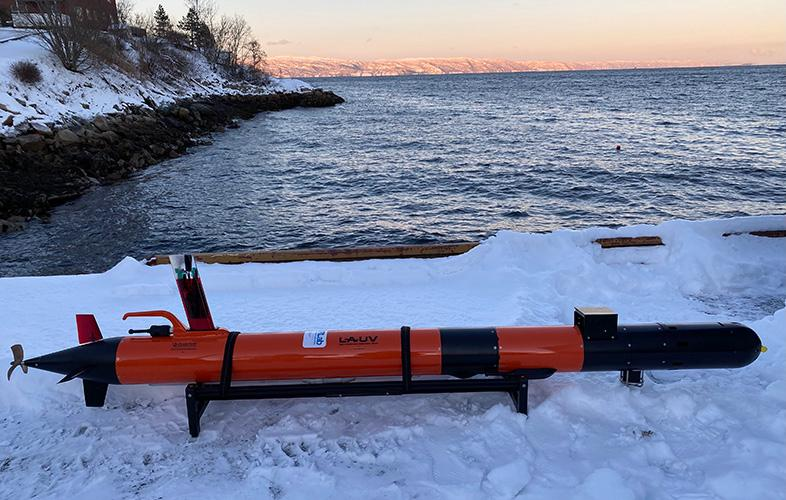
\includegraphics[width = 0.5\columnwidth]{figures/distr_NSB/LAUV-Roald}
    \vspace*{-1mm}
    \caption{Photo of one of the two \glspl{lauv} used in the reported field experiments, courtesy of \url{www.ntnu.edu/aur-lab/}.}
    \label{fig:distr_NSB_LAUV}
    \vspace*{-10mm}
\end{figure}

\begin{figure}[p]
    \begin{minipage}{0.48\textwidth}
        \begin{subfigure}{\textwidth}
            % This file was created by matlab2tikz.
%
%The latest updates can be retrieved from
%  http://www.mathworks.com/matlabcentral/fileexchange/22022-matlab2tikz-matlab2tikz
%where you can also make suggestions and rate matlab2tikz.
%
\definecolor{mycolor1}{rgb}{0.00000,0.44700,0.74100}%
\definecolor{mycolor2}{rgb}{0.85000,0.32500,0.09800}%
%
\begin{tikzpicture}

\begin{axis}[%
width=0.85\textwidth,
height=75mm,
xmin=10.3555,
xmax=10.36,
xtick={10.358333},
xticklabels={$10^{\circ}21.50'$},
tick label style={font=\small},
xlabel style={font=\color{white!15!black},yshift=1.5mm},
xlabel={Longitude},
ymin=63.43465,
ymax=63.4371,
ytick={63.4350,63.4358,63.4367},
yticklabels={$63^{\circ}26.10'$, $63^{\circ}26.15'$, $63^{\circ}26.20'$},
xmajorgrids,
ymajorgrids,
ylabel style={font=\color{white!15!black}},
ylabel={Latitude},
axis background/.style={fill=white},
title style={font=\bfseries,yshift=-2.25mm},
title={Trajectory},
%legend style={/tikz/column 2/.style={column sep=2pt,}, font=\small, at={(1.12,1.08)}, anchor=north east},
%legend columns=1
]
\addplot [color=mycolor1, line width=0.8pt]
  table[]{experiment_nominal_trajectory-1.tsv};
%\addlegendentry{AUV 1}

\addplot[only marks, mark=*, mark options={}, mark size=2.5000pt, draw=mycolor1, fill=mycolor1, forget plot] table[]{experiment_nominal_trajectory-2.tsv};
\addplot [color=mycolor2, line width=0.8pt]
  table[]{experiment_nominal_trajectory-3.tsv};
%\addlegendentry{AUV 2}

\addplot[only marks, mark=*, mark options={}, mark size=2.5000pt, draw=mycolor2, fill=mycolor2, forget plot] table[]{experiment_nominal_trajectory-4.tsv};
\addplot [color=black, line width=0.8pt]
  table[]{experiment_nominal_trajectory-5.tsv};
%\addlegendentry{Path}

\addplot[only marks, mark=square*, mark options={}, mark size=1.8607pt, draw=black, fill=black, forget plot] table[]{experiment_nominal_trajectory-6.tsv};
\end{axis}
\end{tikzpicture}%
            \vspace{-2mm}
            \caption{The trajectory of the AUVs. The markers represent the AUVs at times $t = 0, 60, \ldots, 420$ seconds.}
            \label{fig:distr_NSB_experiment_nominal_trajectory}
        \end{subfigure}

        \vspace{-1mm}

        \begin{subfigure}{\textwidth}
            % This file was created by matlab2tikz.
%
%The latest updates can be retrieved from
%  http://www.mathworks.com/matlabcentral/fileexchange/22022-matlab2tikz-matlab2tikz
%where you can also make suggestions and rate matlab2tikz.
%
\definecolor{mycolor1}{rgb}{0.00000,0.44700,0.74100}%
\definecolor{mycolor2}{rgb}{0.85000,0.32500,0.09800}%
\definecolor{mycolor3}{rgb}{0.92900,0.69400,0.12500}%
\definecolor{mycolor4}{rgb}{0.49400,0.18400,0.55600}%
%
\begin{tikzpicture}

\begin{axis}[%
width=0.8\textwidth,
height=18mm,
scale only axis,
xmin=0,
xmax=450,
xlabel style={font=\color{white!15!black},yshift=1.5mm},
xlabel={Time [s]},
ymin=-0.0004,
ymax=0.0004,
ylabel style={font=\color{white!15!black},yshift=-1.5mm},
ylabel={$\tilde{s}_i$ [--]},
xmajorgrids,
ymajorgrids,
axis background/.style={fill=white},
title style={font=\bfseries},
title={Path parameter errors},
legend style={/tikz/column 2/.style={column sep=2pt,}, font=\small},
legend columns=2
]
\addplot [color=mycolor1, line width=0.8pt]
  table[]{experiment_nominal_parameter-1.tsv};
\addlegendentry{AUV 1}

\addplot [color=mycolor2, line width=0.8pt]
  table[]{experiment_nominal_parameter-2.tsv};
\addlegendentry{AUV 2}

\addplot[only marks, mark=x, mark options={}, mark size=3.000pt, draw=mycolor1, forget plot] table[]{experiment_nominal_parameter-3.tsv};
\addplot[only marks, mark=x, mark options={}, mark size=3.000pt, draw=mycolor2, forget plot] table[]{experiment_nominal_parameter-4.tsv};
\end{axis}

\end{tikzpicture}%
            \vspace{-3mm}
            \caption{The path parameter errors. The markers represent transmissions.}
            \label{fig:distr_NSB_experiment_nominal_parameter}
        \end{subfigure}
    \end{minipage}
    \hspace{\fill}
    \begin{minipage}{0.48\textwidth}

        \hspace*{\fill}
        \begin{subfigure}{\textwidth}
            \hspace*{-5mm}
            % This file was created by matlab2tikz.
%
%The latest updates can be retrieved from
%  http://www.mathworks.com/matlabcentral/fileexchange/22022-matlab2tikz-matlab2tikz
%where you can also make suggestions and rate matlab2tikz.
%
\definecolor{mycolor1}{rgb}{0.00000,0.44700,0.74100}%
\definecolor{mycolor2}{rgb}{0.85000,0.32500,0.09800}%
%
\begin{tikzpicture}

\begin{axis}[%
width=0.8\textwidth,
height=18mm,
at={(0,27mm)},
scale only axis,
xmin=0,
xmax=450,
%xlabel style={font=\color{white!15!black},yshift=1.5mm},
%xlabel={Time [s]},
ymin=-30.2222476170977,
ymax=10,
ylabel style={font=\color{white!15!black},yshift=-1.5mm},
ylabel={$x$ [m]},
xmajorgrids,
ymajorgrids,
axis background/.style={fill=white},
title style={font=\bfseries,yshift=-2.5mm},
title={Formation path-following errors},
legend style={/tikz/column 2/.style={column sep=2pt,}, font=\small},
legend columns=3
]
\addplot [color=mycolor1, line width=0.8pt]
  table[]{experiment_nominal_errors-1.tsv};
%\addlegendentry{$\tilde{\sigma}_1$}

\addplot [color=mycolor2, line width=0.8pt]
  table[]{experiment_nominal_errors-2.tsv};
%\addlegendentry{$\tilde{\sigma}_2$}

\addplot [color=black, line width=0.8pt]
  table[]{experiment_nominal_errors-3.tsv};
%\addlegendentry{$\mat{p}_b^p$}

\end{axis}

\begin{axis}[%
width=0.55\textwidth,
height=8mm,
scale only axis,
at={(0.22\textwidth, 30mm)},
xmin=250,
xmax=450,
ymin=-2.2,
ymax=2.2,
axis background/.style={fill=white},
tick label style={font=\scriptsize},
xticklabel style={yshift=0.5mm},
yticklabel style={xshift=0.5mm},
xmajorgrids,
ymajorgrids,
]
\addplot [color=mycolor1, forget plot, line width=0.8pt]
  table[]{experiment_nominal_errors-4.tsv};
\addplot [color=mycolor2, forget plot, line width=0.8pt]
  table[]{experiment_nominal_errors-5.tsv};
\addplot [color=black, forget plot, line width=0.8pt]
  table[]{experiment_nominal_errors-6.tsv};
\end{axis}

\begin{axis}[%
width=0.8\textwidth,
height=19mm,
scale only axis,
at={(0,0)},
xmin=0,
xmax=450,
xlabel style={font=\color{white!15!black},yshift=1.5mm},
xlabel={Time [s]},
ymin=-12,
ymax=6,
ylabel style={font=\color{white!15!black},yshift=-2mm},
ylabel={$y$ [m]},
xmajorgrids,
ymajorgrids,
axis background/.style={fill=white},
legend style={/tikz/column 2/.style={column sep=2pt,}, font=\small, at={(0.98,1.25)}, anchor=north east},
legend columns=3
]
\addplot [color=mycolor1, line width=0.8pt]
  table[]{experiment_nominal_errors-7.tsv};
\addlegendentry{$\tilde{\bs{\sigma}}_1$}

\addplot [color=mycolor2, line width=0.8pt]
  table[]{experiment_nominal_errors-8.tsv};
\addlegendentry{$\tilde{\bs{\sigma}}_2$}

\addplot [color=black, line width=0.8pt]
  table[]{experiment_nominal_errors-9.tsv};
\addlegendentry{$\mat{p}_b^p$}

\end{axis}

\begin{axis}[%
width=0.55\textwidth,
height=8mm,
scale only axis,
at={(0.22\textwidth, 2.5mm)},
xmin=250,
xmax=450,
ymin=-1.8,
ymax=1.5,
axis background/.style={fill=white},
tick label style={font=\scriptsize},
xticklabel style={yshift=1mm},
yticklabel style={xshift=0.5mm},
xmajorgrids,
ymajorgrids,
]
\addplot [color=mycolor1, forget plot, line width=0.8pt]
  table[]{experiment_nominal_errors-10.tsv};
\addplot [color=mycolor2, forget plot, line width=0.8pt]
  table[]{experiment_nominal_errors-11.tsv};
\addplot [color=black, forget plot, line width=0.8pt]
  table[]{experiment_nominal_errors-12.tsv};
\end{axis}
\end{tikzpicture}%

            \vspace{-3mm}
            \caption{The path-following and formation-keeping errors.}
            \label{fig:distr_NSB_experiment_nominal_errors}
        \end{subfigure}

        %\vspace{-4mm}

        \hspace*{\fill}
        \begin{subfigure}{\textwidth}
            \hspace*{-5mm}
            % This file was created by matlab2tikz.
%
%The latest updates can be retrieved from
%  http://www.mathworks.com/matlabcentral/fileexchange/22022-matlab2tikz-matlab2tikz
%where you can also make suggestions and rate matlab2tikz.
%
\definecolor{mycolor1}{rgb}{0.00000,0.44700,0.74100}%
\definecolor{mycolor2}{rgb}{0.85000,0.32500,0.09800}%
%
\begin{tikzpicture}

\begin{axis}[%
width=0.8\textwidth,
height=15mm,
scale only axis,
at={(0,23mm)},
xmin=0,
xmax=450,
%xlabel style={font=\color{white!15!black},yshift=1.5mm},
%xlabel={Time [s]},
ymin=-2,
ymax=2,
ylabel style={font=\color{white!15!black},yshift=-1.5mm},
ylabel={$x$ [m]},
xmajorgrids,
ymajorgrids,
axis background/.style={fill=white},
title style={font=\bfseries,yshift=-2.5mm},
title={Barycenter estimate errors},
legend style={/tikz/column 2/.style={column sep=2pt,}, font=\small, at={(0.98,0.01)}, anchor=south east},
]
\addplot [color=mycolor1, line width=0.8pt]
  table[]{experiment_nominal_barycenter-1.tsv};
%\addlegendentry{AUV 1}

\addplot [color=mycolor2, line width=1pt, dashed]
  table[]{experiment_nominal_barycenter-2.tsv};
%\addlegendentry{AUV 2}

\end{axis}

\begin{axis}[%
width=0.8\textwidth,
height=15mm,
scale only axis,
at={(0,0)},
xmin=0,
xmax=450,
xlabel style={font=\color{white!15!black},yshift=1.5mm},
xlabel={Time [s]},
ymin=-2,
ymax=3,
ylabel style={font=\color{white!15!black},yshift=-1.5mm},
ylabel={$y$ [m]},
xmajorgrids,
ymajorgrids,
axis background/.style={fill=white},
legend style={/tikz/column 2/.style={column sep=2pt,}, font=\small, at={(0.98,1)}, anchor=north east},
legend columns=2
]
\addplot [color=mycolor1, line width=0.8pt]
  table[]{experiment_nominal_barycenter-3.tsv};
\addlegendentry{AUV 1}

\addplot [color=mycolor2, line width=1pt, dashed]
  table[]{experiment_nominal_barycenter-4.tsv};
\addlegendentry{AUV 2}

\end{axis}

\end{tikzpicture}%
            \vspace{-3mm}
            \caption{The $x$- and $y$-components of barycenter estimate errors.}
            \label{fig:distr_NSB_experiment_nominal_barycenter}
        \end{subfigure}
    \end{minipage}

    \vspace*{-3mm}
    \caption{Results of a nominal experiment.}
    \label{fig:distr_NSB_experiment_nominal}
\end{figure}
